\chapter{Refining Heuristics}
In this chapter are discussed the heuristic that starting from an initial solution of the TSP return a better solution in term of cost. This kind of heuristic will be called Refining Heuristics because of the solution cost improvement. 

\section{2-opt} \label{sec:best_2_opt}

This heuristic is a simple local search algorithm for TSP problem.\\
\texttt{2\_opt()} 
\begin{enumerate}
	\item iterate over each edge of the tour $ (n_1,n_2) \in E, $ with cost $ c_{n_1n_2} $
	\item for each other edge of the tour $ (m_1, m_2) \in E $ with no node in common, $ m_1,m_2 \ne n_1,n_2 $ and associated cost $ c_{m_1m_2} $
	\item evaluate which is the pair of edges that has the best cost improvement $ \delta_{cost} = c_{n_1m_1} + c_{n_2m_2} - c_{n_1n_2} - c_{m_1m_2} $.
\end{enumerate}
In the example in fig \ref{fig:2_opt_graph} the pair that has the best improvement is $ (1,4) $ and $ (5,2) $. Note that although $ (5,2) = (2,5) $ for the model, for this algorithm it must be choose an orientation of the tour, and each edge must be represented with consequent ordered node pair: if $ (1,4) $ is the first considered edge, it impose the orientation of the tour and to calculate $ \delta_{cost} $ according with the formula defined above, the second edge is $ (5,2) $ not $ (2,5) $, and the added edges are $ (1,5) $ and $ (4,2) $. Adding $ (1,2) $ and $ (5,4) $ would create two different tours.


\begin{figure}[h]
	\centering
	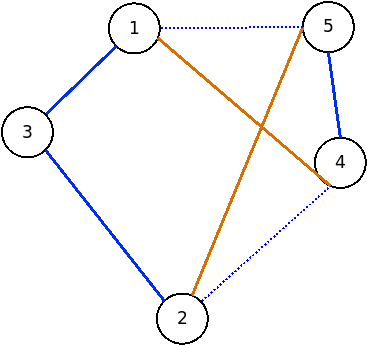
\includegraphics[width=.3\columnwidth]{img/2_opt_graph.png}
	\caption{Example graph to explain \texttt{2\_opt()} method. The input graph is that with continuous edges. \texttt{2\_opt()} would remove $ (1,4) $ and $ (2,5) $ from the tour and replace them with $ (1,5) $ and $  (2,4) $}
	\label{fig:2_opt_graph}
\end{figure}
As can be seen in fig \ref{fig:lb_time_grasp_best_two_opt_d2103} multiple execution of \texttt{2\_opt()} can improve more than 50\% the cost of the solution before to find a local minimum.
\begin{figure}[!h]
\centering
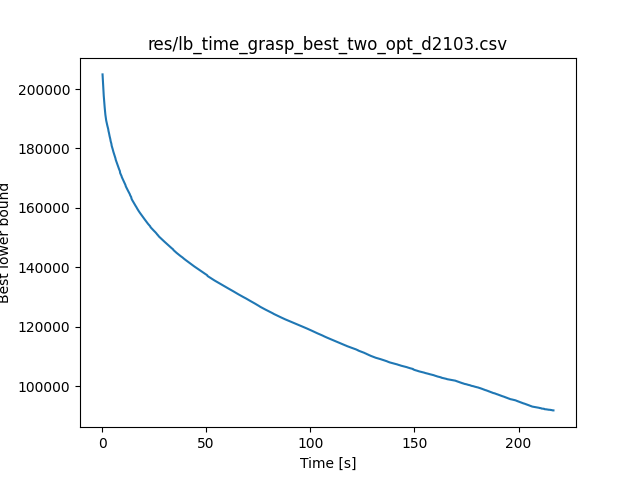
\includegraphics[width=.6\columnwidth]{../res/lb_time_grasp_best_two_opt_d2103.png}
\caption{Consequence execution of \texttt{2\_opt()} until local minimum if found. GRASP constructive heuristic is used to find the first available solution.}
\label{fig:lb_time_grasp_best_two_opt_d2103}
\end{figure}

It is interesting to see the solution cost profile of \texttt{2\_opt()} (fig \ref{fig:a280_25}) applied to the best of the greedy solution. Note that the best tour is calculated in $ 7.42 $s with \texttt{subtour\_callback\_general} but \texttt{2\_opt()} find similar solution in $ 0.07$s

\begin{figure}[!h]
	\begin{subfigure}{.5\columnwidth}
		\centering
		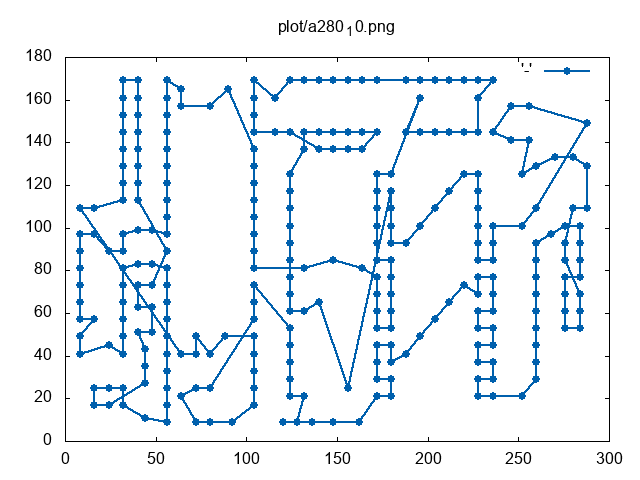
\includegraphics[width=0.9\columnwidth]{../res/a280_10.png}
		\caption{The shortest greedy tours.}
		\label{fig:a280_10}
	\end{subfigure}
	\begin{subfigure}{.5\columnwidth}
		\centering
		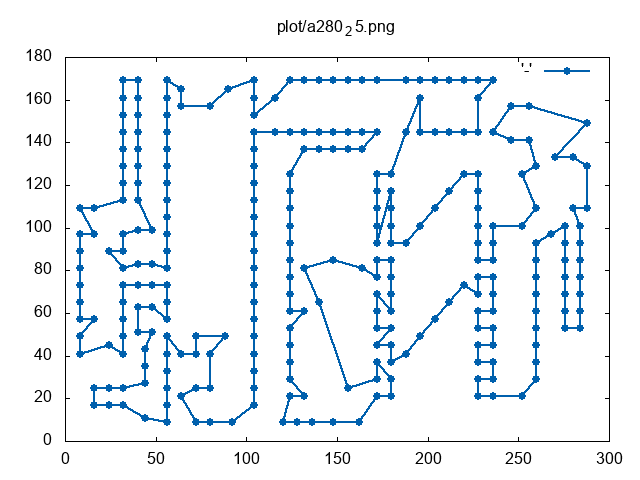
\includegraphics[width=0.9\columnwidth]{../res/a280_25.png}
		\caption{The result of iterative \texttt{2\_opt} applied after a the best greedy.}
		\label{fig:a280_25}
	\end{subfigure}
	\begin{subfigure}{.5\columnwidth}
		\centering
		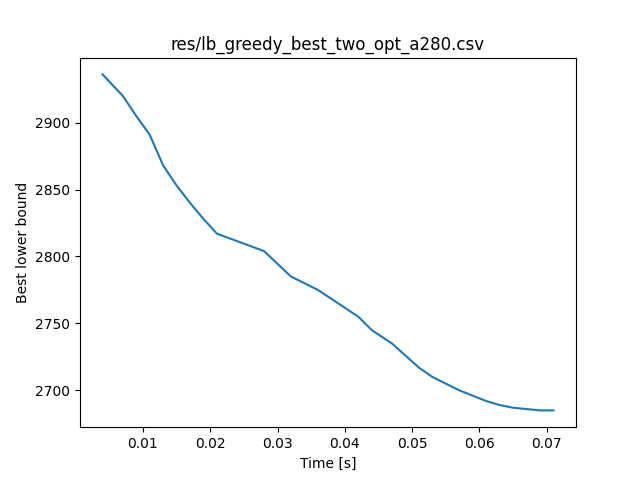
\includegraphics[width=0.9\columnwidth]{../res/lb_greedy_best_two_opt_a280.png}
		\caption{The profile of the solution cost over time of the \texttt{2\_opt} optimization.}
		\label{fig:lb_greedy_best_two_opt_a280}
	\end{subfigure}
	\begin{subfigure}{.5\columnwidth}
		\centering
		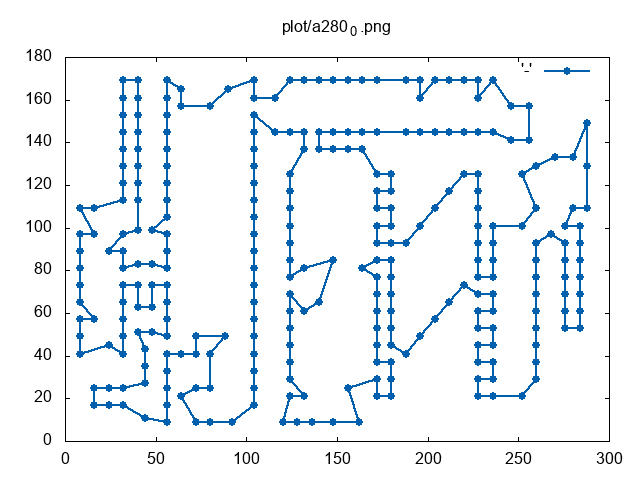
\includegraphics[width=0.9\columnwidth]{../res/a280_0.png}
		\caption{The shortest tour tours.}
		\label{fig:a280_0}
	\end{subfigure}
\end{figure}

